\documentclass[11pt]{article}
\usepackage[letterpaper,margin=.25in]{geometry}
\usepackage{amsmath,amssymb,booktabs,array,tabularx,xcolor,tikz,hyperref,embedfile,microtype}
\usetikzlibrary{trees}
\hypersetup{colorlinks=true,urlcolor=blue!55!black}
\pagestyle{empty}
\setlength{\parindent}{0pt}
\setlength{\parskip}{4pt}
\linespread{1.035}\selectfont
\definecolor{navy}{RGB}{25,54,86}
\definecolor{soft}{RGB}{244,247,250}
\tikzset{branch/.style={circle,draw=navy,line width=.6pt,inner sep=2pt},trueleaf/.style={circle,draw=navy,fill=navy,inner sep=2.1pt},falseleaf/.style={circle,draw=navy,fill=white,inner sep=1.8pt}}
\newcommand{\sectionbar}[1]{\vspace{3pt}{\color{navy}\bfseries #1}\par\vspace{2pt}\hrule\vspace{4pt}}
\begin{document}
\enlargethispage{.12in}

\embedfile[desc={A120591 exact certificate payload},mimetype=application/json]{certificate_payload.json}
{\color{navy}\LARGE\bfseries A120591 concise calculus certificate}\hfill{\small VERIFIED}\\[-1pt]
{\small Bradley Klee, \quad Mech.An.ika Sol (Open AI) \hfill July 31, 2026}

\sectionbar{Definition and first terms}
\(\displaystyle A(x)=A_{\mathrm{parent}}(x)^{3},\quad A_{\mathrm{parent}}(x)=A_{120590}(x)\), with the origin-normalized solution.\\
{\footnotesize Normalization/grammar: \texttt{ordered forest of 3 parent A120590 typogeometries}.}\\
\(a(0),\ldots,a(7)=1,3,12,76,600,5304,50232,498360\).\\[2pt]
{\small Kernel used throughout: \(\displaystyle \rho(u)=u\left(1-3\,u^{1}-1\,u^{2}\right)\), so \(x=\rho(T(x))\).}

\sectionbar{Typogeometry}
\begin{minipage}[t]{.235\textwidth}\centering 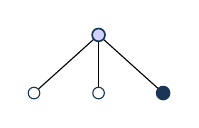
\begin{tikzpicture}[level distance=9mm,level 1/.style={sibling distance=10mm},level 2/.style={sibling distance=6mm},scale=.82,transform shape] \node[branch,fill=blue!18] (n0) {} child {node[falseleaf] (n1) {}} child {node[falseleaf] (n2) {}} child {node[trueleaf] (n3) {}};\end{tikzpicture}\\[2pt]{\normalsize\texttt{\{0,0,1\}x1}}\end{minipage}\begin{minipage}[t]{.235\textwidth}\centering 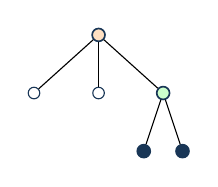
\begin{tikzpicture}[level distance=9mm,level 1/.style={sibling distance=10mm},level 2/.style={sibling distance=6mm},scale=.82,transform shape] \node[branch,fill=orange!24] (n0) {} child {node[falseleaf] (n1) {}} child {node[falseleaf] (n2) {}} child {node[branch,fill=green!20] (n3) {} child {node[trueleaf] (n4) {}} child {node[trueleaf] (n5) {}}};\end{tikzpicture}\\[2pt]{\normalsize\texttt{\{0,0,\{1,1\}\}x3}}\end{minipage}\begin{minipage}[t]{.235\textwidth}\centering 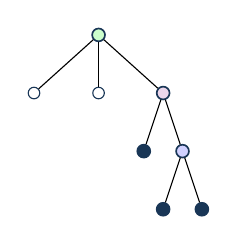
\begin{tikzpicture}[level distance=9mm,level 1/.style={sibling distance=10mm},level 2/.style={sibling distance=6mm},scale=.82,transform shape] \node[branch,fill=green!20] (n0) {} child {node[falseleaf] (n1) {}} child {node[falseleaf] (n2) {}} child {node[branch,fill=violet!16] (n3) {} child {node[trueleaf] (n4) {}} child {node[branch,fill=blue!18] (n5) {} child {node[trueleaf] (n6) {}} child {node[trueleaf] (n7) {}}}};\end{tikzpicture}\\[2pt]{\normalsize\texttt{\{0,0,\{1,\{1,1\}\}\}x9}}\end{minipage}\begin{minipage}[t]{.235\textwidth}\centering 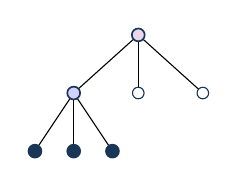
\begin{tikzpicture}[level distance=9mm,level 1/.style={sibling distance=10mm},level 2/.style={sibling distance=6mm},scale=.82,transform shape] \node[branch,fill=violet!16] (n0) {} child {node[branch,fill=blue!18] (n1) {} child {node[trueleaf] (n2) {}} child {node[trueleaf] (n3) {}} child {node[trueleaf] (n4) {}}} child {node[falseleaf] (n5) {}} child {node[falseleaf] (n6) {}};\end{tikzpicture}\\[2pt]{\normalsize\texttt{\{\{1,1,1\},0,0\}x1}}\end{minipage}

{\footnotesize forest slots are explicit; 0 denotes an empty slot. Filled endpoints are true leaves; open endpoints are false/empty leaves. For colored grammars, color is genuine constructor data and is not silently converted into a positional zero pattern.}

{\footnotesize Typogeometric constructor codes and multiplicities: \(\Delta_{2}\!:\,3,\;\Delta_{3}\!:\,1\).}

\sectionbar{Coefficient and contour extraction}
{\footnotesize \[\begin{gathered}p(n)=[x^n]A_{\rm parent}(x),\\a(n)=\sum_{\substack{n_1,\ldots,n_3\ge0\\n_1+\cdots+n_3=n}}\prod_{j=1}^{3}p(n_j).\end{gathered}\]}
\([x^n]A(x)^{3}=\dfrac{3}{2\pi i n}\oint_\gamma\dfrac{(1+u)^{2}\,du}{u^nD(u)^n}.\)

\sectionbar{Recurrence}
{\footnotesize \(\sum_{r=0}^{3}P_r(n)a(n+r)=0\), \(n\ge 1\), with \[\begin{aligned}P_{0}(n)&=0\\P_{1}(n)&=-27\,n^{2} - 54\,n - 24\\P_{2}(n)&=-162\,n^{2} - 567\,n - 486\\P_{3}(n)&=13\,n^{2} + 65\,n + 78\end{aligned}\]}

\sectionbar{Differential equation}
{\footnotesize \[\left(3\,x^{2}\right)A(x)+\left(-27\,x^{3} - 81\,x^{2}\right)A'(x)+\left(-27\,x^{4} - 162\,x^{3} + 13\,x^{2}\right)A^{(2)}(x)=24\,x^{3} + 72\,x^{2}.\]}

\sectionbar{Matrices, telescoper certificate, and checks}
{\small \(\text{No compact matrix tuple is shown; see the embedded exact reduction data.}\)}
\par\vspace{6pt}
{\small\textbf{Certificate.}\par\smallskip\(\displaystyle R(n,u)=N(n,u)/(-u^{3} - 3\,u^{2} + u)^{2}.\)\par}
\vspace{4pt}
{\small Telescoping identity: \(\sum_r P_r(n)H_{n+r}(u)=\partial_u\!\left(R(n,u)H_n(u)\right).\)\par}
\vspace{4pt}
{\footnotesize Matrix dimensions: \(6\times 6\); remainder \(3\times 4\), rank 3, nullity 1. The exact telescoping residual is zero. The recurrence reconstructs all 24 stored terms; 6/6 published OEIS prefix terms match.\par}

\vfill
\colorbox{soft}{\parbox{.97\textwidth}{\tiny Canonical records: \texttt{data/tree\_model.json}, \texttt{data/contour.json}, \texttt{data/matrices.json}, \texttt{data/recurrence.json}, \texttt{data/ode.json}. Embedded payload contains exact sources and SHA-256 matrix identifiers. Compare with the verbose certificate for A120590.}}
\end{document}
